\section{Introdução} 
\label{introduction}
\subsection{Definição dos objetivos e da sua relevância}
A palavra ``computador'' é usada desde o século XVII, tendo a sua primeira referência escrita datada de 1613. No entanto, por muito tempo ``computador'' não tinha o mesmo significado que tem hoje, sendo utilizado, até a década de 1940, para se referir à profissão de alguém que calcula, segundo o dicionário Michaelis: ``Aquele ou aquilo que calcula baseado em valores digitais; calculador, calculista'' \cite{4}.

Tendo em vista o antigo significado atribuído à palavra ``computador'', pode-se questionar sobre como uma palavra antes atribuída às pessoas, passa a se referir a máquinas. Isso tem a ver, em ordem cronológica, com o estudo de Alan Turing (Reino Unido, 1912-1954) – um matemático, lógico, criptógrafo e herói de guerra – que tinha como objetivo compreender aquilo que podia ou não ser calculado, resultando no modelo mais poderoso de computador – a Máquina da Turing, – também conhecida como ``Maquina Universal''. Ao lermos o termo ``Máquina de Turing'' logo vem à nossa mente a figura de um computador, mas engana-se quem pensa isso – a Máquina de Turing nada mais é que uma fórmula matemática, ou um conceito abrangente, que fundamenta o pensamento computacional. Esse trabalho, publicado em 1937, trouxe muitas contribuições para o desenvolvimento da computação, e observamos isso na influência dele em computadores e celulares que você, leitor, pode estar usando para ler esse  trabalho.  

A Máquina de Turning será o ponto de início desse trabalho, dada a sua importância e contribuição para a computação – tanto em sua constituição como em seu funcionamento. 

O modelo matemático da Máquina de Turing foi desenvolvido a partir de três principais componentes: fita infinita; cabeçote; e a máquina de estado finito; – sendo similar a um autômato finito\footnote{Um sub-tópico da Ciência da computação teórica, também chamado máquina de estados finita determinística — é uma máquina de estados finita que aceita ou rejeita cadeias de símbolos gerando um único ramo de computação para cada cadeia de entrada.}, porém com uma memória ilimitada e irrestrita, ilustrada na figura \ref{turing_machine} abaixo.

\vspace{1cm}
\begin{figure}[H] \centering 
  \makebox[\textwidth][c]{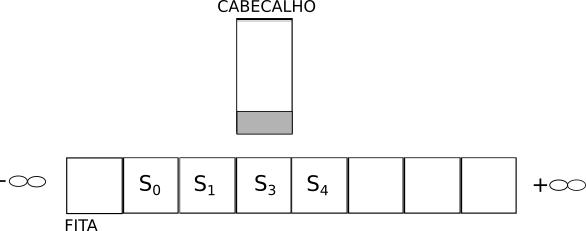
\includegraphics[width=0.8\textwidth]{turing_machine.png}}
  \caption{\label{turing_machine} Desenho esquemático Máquina de Turing} 
\end{figure}

Neste modelo, a fita infinita é dividida em células, cada uma contendo um símbolo de um alfabeto finito. O cabeçote é responsável por se deslocar para a direita ou para a esquerda e efetuar a leitura ou escrita em uma célula. Este processo é ilustrado pelo Prof. Dr. Fabio Gagliardi Cozman \cite{7} da seguinte forma:

\begin{enumerate}
  \item Inicialmente a fita contém somente a cadeia de entrada (dados originários do programa), disposta no ``meio''\footnote{Meio é algo abstrato nesse sentido, pois não existe meio de um valor infinito} da fita, com o cabeçote posicionado no início da cadeia, tendo o resto das células da fita vazias;
  \item Para armazenar algo, a máquina escreve na fita;
  \item O cabeçote pode ser movido livremente para a esquerda ou direita, afim de ler ou escrever valores em qualquer célula;
  \item As saídas ``aceita'' e ``rejeita'' são obtidas ao entrar nos estados de aceitação e rejeição;
  \item Se não entrar em um estado de aceitação ou rejeição, continuará sua computação para sempre, em ``loop infinito''.
\end{enumerate}

Assim, a partir desse funcionamento, o modelo computacional de Turing possibilitou três operações fundamentais básicas: a leitura, a escrita e a movimentação.   

Após aproximadamente uma década, em 1946, esse conceito foi implementado pela primeira vez, no primeiro computador digital eletrônico de grande escala, criado pelos cientistas norte-americanos, John Presper Eckert e John W. Mauchly, da Electronic Control Company. Chamado de ENIAC (Electrical Numerical Integrator and Calculator), essa máquina foi mais um marco da evolução da tecnologia. Em 1956, ao final dos seus 10 anos de operação, e com constantes aprimoramentos, o ENIAC continha 20.000 tubos de vácuo, 7.200 diodos de cristal, 1.500 relés, 70.000 resistores, 10.000 capacitores e aproximadamente 5.000.000 juntas soldadas à mão. Ele pesava mais de 27 toneladas, tinha aproximadamente 2,4m × 0,9m × 30m, consumia 150 kW de eletricidade e ocupava 167 m² \cite{2}, tendo a sua disposição ilustrada na figura \ref{ENIAC_floor_layout} abaixo. 

\vspace{1cm}
\begin{figure}[H] \centering 
 \makebox[\textwidth][c]{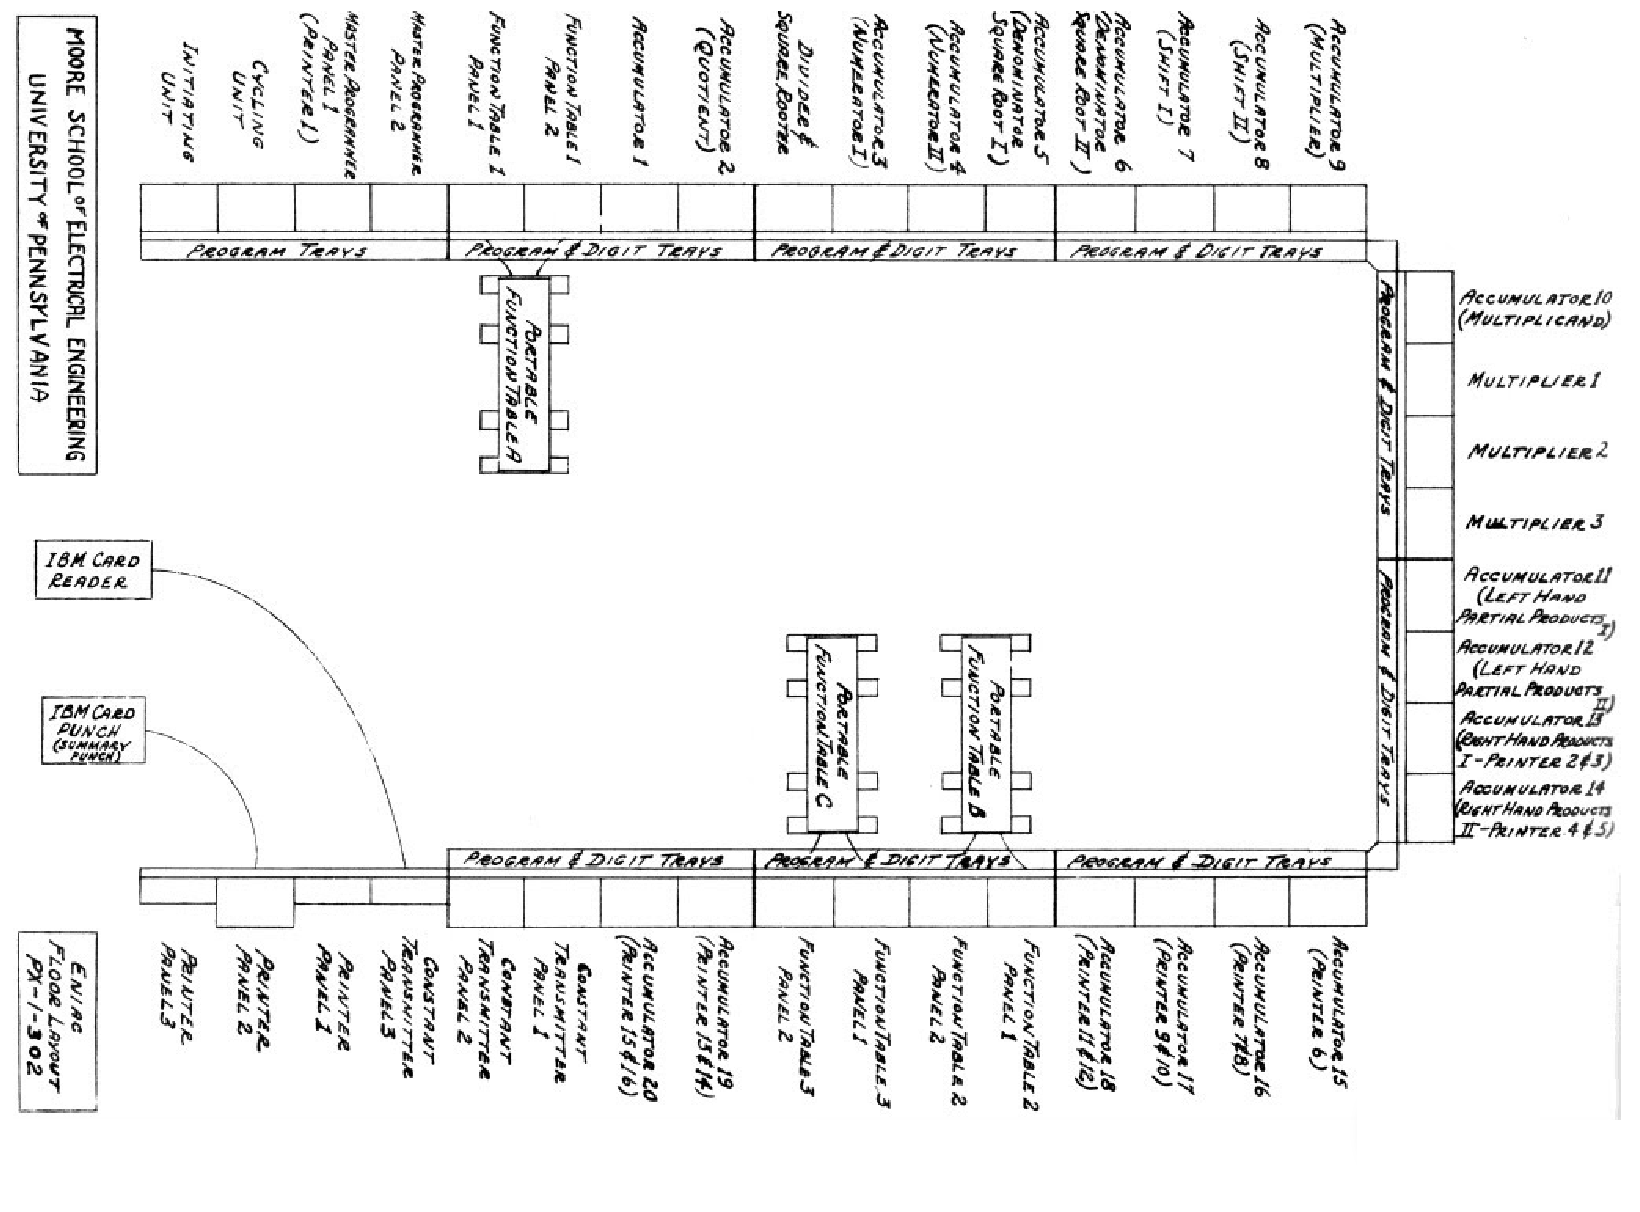
\includegraphics[width=0.8\textwidth]{ENIAC_floor_layout.png}}
  \caption{\label{ENIAC_floor_layout} Desenho esquemático do ENIAC/US Center for Military History — Adele Goldstine} 
\end{figure}

A partir do ENIAC, as possibilidades tecnológicas tomaram uma nova proporção e em 1969, apenas 13 anos após o desligamento do primeiro computador digital eletrônico, surge o computador de bordo da Apollo 11 — na missão que levou o homem à Lua. O Apollo Guidance Computer, uma revolução no mundo computacional, era bem menor do que o seu antecessor e tinha 32.768 bits\footnote{Para uma explicação elaborada sobre bits refira-se ao capítulo \ref{classic_comp} pagina \pageref{bits}} de RAM, o suficiente para armazenar apenas um texto não formatado, com cerca de 2.000 palavras.

Ponto de interesse: O que contrasta o Iphone XS com 4gb de RAM lançado em 2018 ao Apollo Guidance Computer de 1969 é que o equipamento mais novo tem cerca de 1 milhão de vezes  mais memória do que aquele que estava no Apollo 11 \cite{5}.

Durante o século XX, além do aumento do poder computacional dos dispositivos, outro fator impactante foi a refatoração de seus tamanhos. Assim, com tecnologias wearables\footnote{A tecnologia em questão não somente pode ser usada como uma peça de roupa ou um acessório, como também tem que possuir características que a conectem a outros aparelhos ou à internet.}, os computadores se tornam ativamente presentes no cotidiano. 

Levando em consideração o rápido avanço e desenvolvimento computacional, entende-se que os computadores trazem benefícios à sociedade, seja facilitando a comunicação e o compartilhamento de conhecimentos, assim como em vários outros aspectos. No entanto, a agilidade dessas \textbf{transformações da tecnologia da computação}, gera grandes expectativas e incertezas sobre o que ainda está por vir, tanto nas questões de mudanças tecnológicas quanto no impacto que trará para a sociedade, principalmente no que se refere à segurança das informações. 

Tendo em vista a incerteza que acompanha o futuro da computação e de seus próximos avanços, a presente pesquisa se propõe a estudar os conceitos da física clássica e da física quântica aplicados à computação, além do estudo dos princípios da criptografia\footnote{Criptografia é um sistema de algoritmos matemáticos que codificam dados para que só o destinatário possa ler.}. Com base nesses conceitos será prototipado um computador clássico de 8 bits em hardware usando apenas portas lógicas simples, de forma a possibilitar uma ilustração clara do funcionamento. Junto a isso será desenvolvida uma aplicação web que ilustra o funcionamento de um processador quântico. Ao final, conceitos de criptografia serão utilizados para exemplificar possíveis mudanças sociais que os próximos avanços tecnológicos podem gerar.

\subsection{Organização do texto}
Essa seção apresenta como está organizado o fluxo de informações dentro deste projeto. Cada capítulo busca se aprofundar no seu específico tema, mantendo a fluidez de idéias e linha de organização do projeto. São os capítulos:

\begin{itemize}
  \item Introdução ( Capitulo \ref{introduction}): Apresenta a história da computação e as abordagens atuais para sanar tais desafios. É nesse capítulo que a introdução ao projeto é feita, contemplando os aspectos históricos e técnicas iniciais da discussão: computadores clássicos e computadores quânticos. Apesar de ter uma abordagem atenua, introduz os temas dos demais capítulos;
  \item Metodologia ( Capitulo \ref{methodologies}): Para a melhor compreensão do tema em discussão, esse capítulo adentrará as metodologias a serem implementadas ao decorrer do projeto, sendo elas: Project Based Learning (PBL) e revisão bibliográfica. Essas instigam o estudo didático através da leitura de pesquisas, livros e artigos, bem como o protagonismo do fazer através da implementação de projetos.
  \item Computador Clássico ( Capitulo \ref{classic_comp}): Compreender a direção em que a tecnologia da computação está caminhando requer um entendimento aprofundado dos avanços que já foram realizados. Assim, neste capítulo será explorado a história do computador partindo do estudo de 1936 de Alan Turing e se desenvolvendo até a finalização de uma implementação de um simulador web simples.
  \item Computador Quântico ( Capitulo \ref{quantum_comp}): Com o pressuposto que a Computação Quântica inaugura toda uma nova geração de computadores, o capítulo 4 apresenta uma trajetoria detalhada dessa jornada percorrendo sua história, arquitetura, algumas implementações, dificuldades e impactos no mundo real.
  \item Computador ( Capitulo \ref{computer}): Construir um computador é por si só um grande desafio. A fim, de melhorar os conhecimentos e também praticar a metodologia PBL, conforme apresentado no capítulo de metodologia. Neste capítulo é apresentado um computador funcional que está sendo construindo neste projeto. É um computador de 8bits que possui todos as principais partes de um computador contemporâneo clássico.
  \item Simulador ( Capitulo \ref{simulator}): Tendo em vista que a física quântica aplicada a computação implementa conceitos altamente abstratos, o simulador quântico tem como propósito principal facilitar a compreensão desses através de uma ferramenta didática e interativa.
  \item Criptografia ( Capitulo \ref{criptography}): Com a possibilidade funcional do computador quântico, novos desafios aparecem e dentre eles diversos na área de criptografia. Neste capítulo é apresentado os desafios impostos a uma área de ampla aplicabilidade industrial e comercial na sociedade que pode sucumbir com a inovação quântica. Logo, é neste capítulo que são apresentados e ilustrados o funcionamento da área, assim bem como, quais os desafios impostos pela inovação quântica.
  \item Próximos passos: 
  \item Impactos Sociais ( Capitulo \ref{social_impacts}): Além da área específica de criptográfica, a computação quântica há de impactar dado forma como a sociedade hoje se organiza, pois, dentre sua aplicabilidade está a possibilidade de otimização em tempo hábil de diversos problemas computacionais, que geram impactos diretos na forma como produtos, mercadorias e serviços são prestados. Neste capítulo tais vislumbramentos e perspectivas serão exercitados.
\end{itemize}

\newpage

